\chapter{MDL and the Occam's Razor in Deep Learning}
\label{ch:mdl_occam}

\section{The Principle of Parsimony}

The fundamental challenge of machine learning is generalization: the ability of a model to perform well on unseen data. At the heart of our understanding of generalization lies the principle of parsimony, most famously articulated as Occam's Razor by the 14th-century philosopher William of Ockham: \textit{``Numquam ponenda est pluralitas sine necessitate''} (Plurality must never be posited without necessity). In the context of statistical modeling and deep learning, Occam's Razor asserts that among competing models that fit the training data equally well, the simplest one is most likely to capture the true underlying data-generating process, and thus most likely to generalize.

The Minimum Description Length (MDL) principle, introduced by Jorma Rissanen in 1978, provides a rigorous, information-theoretic formalization of Occam's Razor. The MDL principle equates learning with data compression: the best model for a given dataset is the one that permits the greatest compression of the data, including the cost of describing the model itself. By viewing learning through the lens of coding theory, MDL escapes the need for arbitrary complexity penalties and grounds model selection in the universal currency of bits.

In classical statistics, MDL is intuitively appealing. For simple parametric models, complexity is often equated with the number of parameters. However, the application of MDL to modern deep learning presents a profound paradox. Modern neural networks $f_\theta$ are massively overparameterized, often possessing more parameters than there are training examples in the dataset $\mathcal{D}$. A naive application of parameter-counting would suggest that these models have an astronomically high description length, leading to catastrophic overfitting. Yet, in practice, these overparameterized models generalize exceptionally well. 

Resolving this paradox requires a more sophisticated understanding of model complexity than mere parameter counting. The true description length of a neural network is not just the number of weights, but the number of bits required to specify those weights to a sufficient precision, such that the model can still accurately reproduce the labels $\mathcal{Y}$ from the inputs $\mathcal{X}$. This realization bridges the gap between information theory, Bayesian inference, and the geometry of the loss landscape. It suggests that deep neural networks are not actually ``complex'' in the MDL sense; rather, the optimization process naturally gravitates towards ``simple'' models---those characterized by flat minima, low-precision weights, and high compressibility.

This chapter delves into the mathematical core of the MDL principle as it applies to deep learning. We will formalize the two-part code, explore its equivalence with Bayesian inference and PAC-Bayesian bounds, and investigate how the geometry of the parameter space dictates the true informational cost of a neural network.

\section{Formalizing MDL: The Two-Part Code}

The simplest formulation of the MDL principle is the \textit{two-part code}. Suppose we wish to transmit the labels $Y = (y_1, \dots, y_N)$ of a dataset $\mathcal{D}$ to a receiver who already possesses the inputs $X = (x_1, \dots, x_N)$. We can achieve this by first transmitting a neural network parameterized by $\theta$, and then transmitting the labels using the network's predictions.

The total description length $L(\mathcal{D}, \theta)$ is the sum of two terms:
\begin{equation}
    L(\mathcal{D}, \theta) = L(\theta) + L(\mathcal{D} \mid \theta)
\end{equation}
where $L(\theta)$ is the code length in bits required to describe the model parameters, and $L(\mathcal{D} \mid \theta)$ is the code length in bits required to describe the data given the model. The MDL principle dictates that we should select the parameters $\theta^*$ that minimize this total length:
\begin{equation}
    \theta^* = \arg\min_\theta \left( L(\theta) + L(\mathcal{D} \mid \theta) \right).
\end{equation}

\subsection{The Cost of Encoding Data}

According to Shannon's source coding theorem, the optimal code length for a sequence of symbols drawn from a distribution $P$ is given by its negative log-likelihood. Thus, the description length of the data given the model is:
\begin{equation}
    L(\mathcal{D} \mid \theta) = -\sum_{i=1}^N \log_2 P(y_i \mid x_i, \theta).
\end{equation}
In the context of deep learning, this term is precisely the empirical risk (or loss) $\mathcal{L}(\theta)$ when using a cross-entropy or mean squared error loss (suitably scaled). For example, if $P(y_i \mid x_i, \theta)$ is a Gaussian distribution $\mathcal{N}(f_\theta(x_i), \sigma^2)$, then $L(\mathcal{D} \mid \theta)$ is proportional to the mean squared error.

\subsection{The Cost of Encoding Parameters}

The model complexity term $L(\theta)$ is more intricate. Since the parameters $\theta \in \mathbb{R}^d$ are continuous, specifying them with infinite precision would require an infinite number of bits. In practice, parameters must be quantized to a finite precision. 

Let us define a prior distribution $P(\theta)$ over the parameter space. We discretize the parameter space into bins of volume $\Delta \theta$. The probability mass of a bin centered at $\theta$ is approximately $P(\theta) \Delta \theta$. The number of bits required to encode this discretized parameter is:
\begin{equation}
    L(\theta) = -\log_2 \left( P(\theta) \Delta \theta \right) = -\log_2 P(\theta) - \log_2 \Delta \theta.
\end{equation}
Here, $- \log_2 P(\theta)$ penalizes parameters that are highly improbable under the prior, while $- \log_2 \Delta \theta$ represents the cost of precision. A smaller $\Delta \theta$ (higher precision) requires more bits. 

\begin{figure}[htbp]
\centering
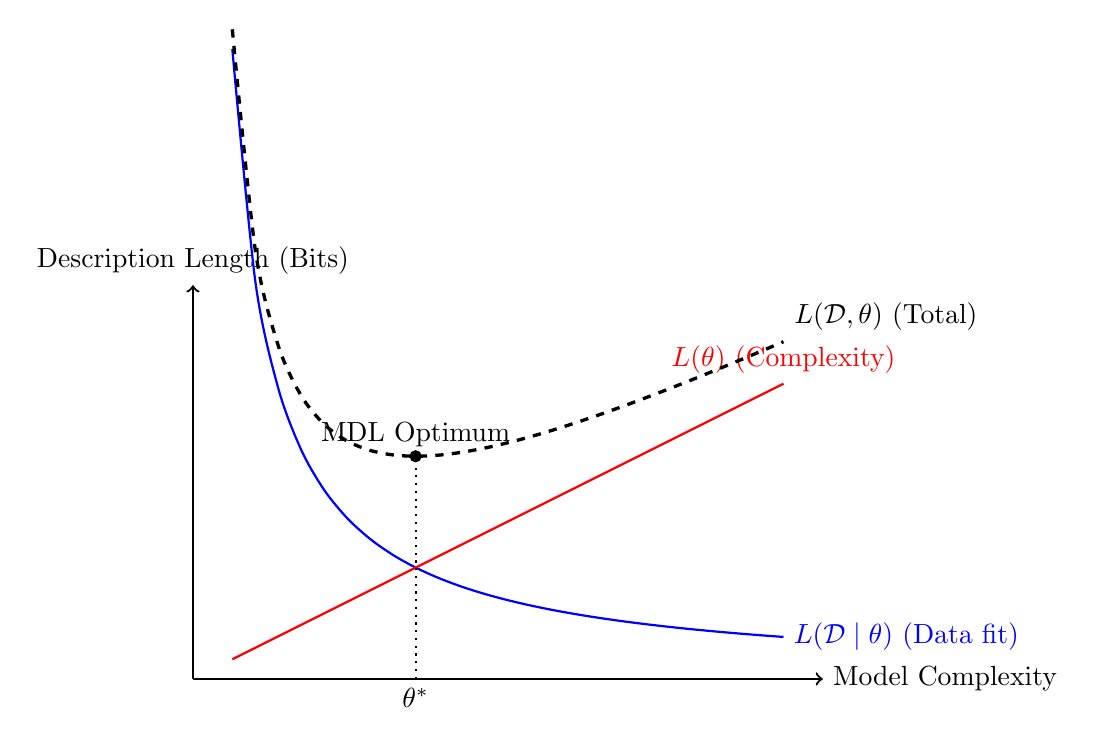
\begin{tikzpicture}[scale=1.0]
    % Axes
    \draw[->, thick] (0,0) -- (8,0) node[right] {Model Complexity};
    \draw[->, thick] (0,0) -- (0,5) node[above] {Description Length (Bits)};
    
    % Curves
    \draw[domain=0.5:7.5, smooth, variable=\x, blue, thick] plot ({\x}, {4/\x}) node[right] {$L(\mathcal{D} \mid \theta)$ (Data fit)};
    \draw[domain=0.5:7.5, smooth, variable=\x, red, thick] plot ({\x}, {0.5*\x}) node[above] {$L(\theta)$ (Complexity)};
    \draw[domain=0.5:7.5, smooth, variable=\x, black, very thick, dashed] plot ({\x}, {4/\x + 0.5*\x}) node[above right] {$L(\mathcal{D}, \theta)$ (Total)};
    
    % Minimum point
    \draw[dotted, thick] (2.828, 0) -- (2.828, 2.828);
    \filldraw (2.828, 2.828) circle (2pt) node[above] {MDL Optimum};
    \node[below] at (2.828, 0) {$\theta^*$};
\end{tikzpicture}
\caption{The MDL trade-off. As model complexity increases, the code length of the data (error) decreases, but the code length of the parameters increases. The MDL principle selects the minimum of the combined cost.}
\label{fig:mdl_tradeoff}
\end{figure}

\subsection{Bayesian Interpretation and PAC-Bayes Bounds}

The two-part MDL framework is closely related to Bayesian inference. Minimizing $L(\mathcal{D}, \theta)$ is mathematically equivalent to maximizing the posterior probability $P(\theta \mid \mathcal{D})$:
\begin{equation}
    P(\theta \mid \mathcal{D}) = \frac{P(\mathcal{D} \mid \theta) P(\theta)}{P(\mathcal{D})}.
\end{equation}
Taking the negative base-2 logarithm yields:
\begin{equation}
    -\log_2 P(\theta \mid \mathcal{D}) = -\log_2 P(\mathcal{D} \mid \theta) - \log_2 P(\theta) + \log_2 P(\mathcal{D}).
\end{equation}
Since $P(\mathcal{D})$ is independent of $\theta$, maximizing the posterior is equivalent to minimizing the description length. However, modern deep learning typically relies on stochastic, rather than deterministic, networks. This leads us to the PAC-Bayesian framework, which provides rigorous generalization bounds aligned with MDL.

Let $Q(\theta)$ be a posterior (or "Gibbs") distribution over the weights, and $P(\theta)$ be a prior. The expected description length of the data under $Q$ is $\mathbb{E}_{\theta \sim Q}[L(\mathcal{D} \mid \theta)]$. The cost of encoding the model is given by the Kullback-Leibler divergence $D_{\text{KL}}(Q \parallel P)$, which represents the excess bits required to code samples from $Q$ using a code optimized for $P$.

\begin{theorem}[PAC-Bayesian MDL Bound (McAllester, 1999)]
Let $\mathcal{L}_{\text{train}}(f_\theta)$ be the empirical error on a dataset of size $N$, and $\mathcal{L}_{\text{test}}(f_\theta)$ be the true expected error. For any prior $P$ independent of the training data, and any $\delta \in (0, 1)$, with probability at least $1 - \delta$ over the choice of the dataset $\mathcal{D}$:
\begin{equation}
    \mathbb{E}_{Q}[\mathcal{L}_{\text{test}}(f_\theta)] \le \mathbb{E}_{Q}[\mathcal{L}_{\text{train}}(f_\theta)] + \sqrt{\frac{D_{\text{KL}}(Q \parallel P) + \ln(N / \delta)}{2N}}.
\end{equation}
\end{theorem}
\begin{proof}
The proof relies on the Donsker-Varadhan variational representation of the Kullback-Leibler divergence. For any measurable function $\phi(\theta)$, it holds that:
\begin{equation}
    \mathbb{E}_Q[\phi(\theta)] \le D_{\text{KL}}(Q \parallel P) + \ln \mathbb{E}_P[e^{\phi(\theta)}].
\end{equation}
Let $\phi(\theta) = 2N (\mathcal{L}_{\text{test}}(f_\theta) - \mathcal{L}_{\text{train}}(f_\theta))^2$. By applying Hoeffding's inequality, one can bound the moment generating function $\mathbb{E}_P[e^{\phi(\theta)}]$. Specifically, for a fixed $\theta$, the probability that the empirical risk deviates from the true risk is bounded exponentially in $N$. Integrating over the prior $P$ and applying Markov's inequality to handle the confidence parameter $\delta$ yields the desired bound after algebraic manipulation. The term $D_{\text{KL}}(Q \parallel P)$ acts precisely as the model complexity penalty $L(\theta)$ in the MDL framework.
\end{proof}

This theorem provides a profound insight: generalization is not guaranteed by having a small number of parameters, but by finding a posterior $Q$ that fits the data well while remaining ``close'' to the prior $P$ in terms of KL divergence. In bits, this means the model can be communicated efficiently.

\subsection{Parameter Precision and Flat Minima}

We now address the apparent contradiction of overparameterization. How can a model with billions of parameters have a small description length? The answer lies in the precision $\Delta \theta$ required to specify the parameters. 

If a neural network converges to a \textit{sharp minimum}, even a tiny perturbation of the weights will drastically increase the loss. To maintain performance, the weights must be specified with exceedingly high precision (a small $\Delta \theta$). This incurs a massive description length penalty $-d \log_2 \Delta \theta$, where $d$ is the number of parameters.

Conversely, if the network converges to a \textit{flat minimum}, the loss is relatively insensitive to perturbations in the weights. We can therefore afford to specify the weights with low precision (a large $\Delta \theta$). The volume of the region in parameter space that yields good performance is large.

\begin{figure}[htbp]
\centering
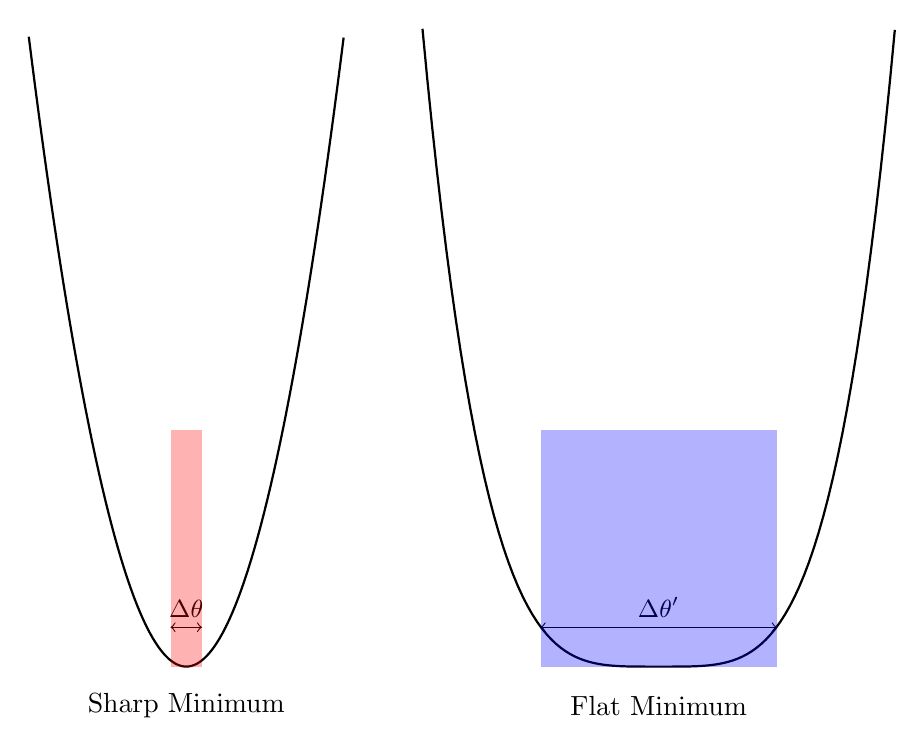
\begin{tikzpicture}
    % Sharp minimum
    \draw[thick, domain=-2:2, samples=100] plot ({\x-3}, {2*\x*\x + 1});
    \node at (-3, 0.5) {Sharp Minimum};
    \draw[<->] (-3.2, 1.5) -- (-2.8, 1.5) node[midway, above] {\small $\Delta \theta$};
    \fill[red, opacity=0.3] (-3.2, 1) rectangle (-2.8, 4);

    % Flat minimum
    \draw[thick, domain=-3:3, samples=100] plot ({\x+3}, {0.1*\x*\x*\x*\x + 1});
    \node at (3, 0.5) {Flat Minimum};
    \draw[<->] (1.5, 1.5) -- (4.5, 1.5) node[midway, above] {\small $\Delta \theta'$};
    \fill[blue, opacity=0.3] (1.5, 1) rectangle (4.5, 4);

\end{tikzpicture}
\caption{Sharp vs. Flat Minima. A sharp minimum (left) requires high precision (small $\Delta \theta$) to remain near the optimal loss, incurring a high description length. A flat minimum (right) tolerates lower precision (large $\Delta \theta'$), resulting in a highly compressible model with a lower description length.}
\label{fig:minima}
\end{figure}

\begin{lemma}[Description Length of a Gaussian Posterior]
Let the prior be an isotropic Gaussian $P(\theta) = \mathcal{N}(0, \sigma_p^2 I)$. Let the approximate posterior $Q$ around a minimum $\theta^*$ be Gaussian $Q(\theta) = \mathcal{N}(\theta^*, \Sigma)$, where $\Sigma = H^{-1}$ and $H$ is the Hessian of the loss landscape at $\theta^*$. The description length (KL divergence) is given by:
\begin{equation}
    D_{\text{KL}}(Q \parallel P) = \frac{1}{2} \left( \frac{\|\theta^*\|^2}{\sigma_p^2} + \text{Tr}\left(\frac{\Sigma}{\sigma_p^2}\right) - d + \ln \left( \frac{| \sigma_p^2 I |}{|\Sigma|} \right) \right).
\end{equation}
\end{lemma}
\begin{proof}
By direct substitution of the Gaussian density functions into the definition of the KL divergence:
$D_{\text{KL}}(Q \parallel P) = \mathbb{E}_{\theta \sim Q}[\ln Q(\theta) - \ln P(\theta)]$. The entropy of $Q$ is $\frac{1}{2}\ln( (2\pi e)^d |\Sigma| )$. The cross-entropy is $-\mathbb{E}_Q[\ln P(\theta)] = \frac{d}{2}\ln(2\pi\sigma_p^2) + \frac{1}{2\sigma_p^2} \mathbb{E}_Q[\|\theta\|^2]$. Using $\mathbb{E}_Q[\|\theta\|^2] = \|\theta^*\|^2 + \text{Tr}(\Sigma)$, the result follows immediately.
\end{proof}

The term $\ln(1/|\Sigma|) = \ln |H|$ demonstrates that sharper minima (larger determinant of the Hessian $H$) linearly increase the description length. The MDL principle thus formally favors flat minima, explaining why heavily regularized optimization trajectories (such as those induced by SGD) yield models that generalize well despite overparameterization.

\subsection{Numerical Example: Quantization and MDL}

Consider a simple binary classification task with $N=1000$ samples. We train a linear classifier with $d=10$ parameters, and a small neural network with $d=1000$ parameters. 
Assume the prior is uniform over a bounded region, and we quantize the weights to $k$ bits per parameter. The complexity term is $L(\theta) = k \cdot d$ bits.

\begin{itemize}
    \item \textbf{Linear Model:} Suppose $k=16$ bits per weight is required to achieve $90\%$ accuracy (error rate $0.1$). The cost of the parameters is $16 \times 10 = 160$ bits. The cost of the data (ignoring the exact entropy formula for simplicity, bounding it via binary entropy) is roughly $N \cdot H(0.1) \approx 1000 \times 0.469 = 469$ bits. Total MDL = 629 bits.
    \item \textbf{Neural Network:} Suppose the neural network achieves $98\%$ accuracy (error rate $0.02$). The cost of the data is $1000 \times H(0.02) \approx 1000 \times 0.141 = 141$ bits. If we use $k=16$ bits, the parameter cost is $16,000$ bits, yielding an MDL of 16,141 bits. The MDL principle would reject this model. However, because the network is overparameterized and sits in a flat minimum, we can aggressively quantize the weights. If we can quantize the weights to $k=0.2$ bits on average (via techniques like pruning and weight sharing) without increasing the error, the parameter cost drops to $200$ bits. The new total MDL is $200 + 141 = 341$ bits. 
\end{itemize}

This numerical illustration underscores that a massive neural network can indeed have a smaller true description length than a simple linear model, provided it is sufficiently compressible.

\begin{horizon}
While the PAC-Bayesian formulation of MDL elegantly explains the generalization of neural networks through the lens of flat minima, several profound mysteries remain. It is conjectured that Stochastic Gradient Descent (SGD), particularly with specific hyperparameter regimes (large learning rates, small batch sizes), acts as an implicit variational inference algorithm that explicitly minimizes the description length. However, a rigorous proof demonstrating that SGD's stationary distribution perfectly aligns with the optimal MDL code remains an open question. 

Furthermore, estimating the true description length (or the determinant of the Hessian $H$) of modern architectures like billion-parameter transformers is computationally prohibitive. Future work might show whether highly scalable approximations of the description length can be used directly as a differentiable regularizer during training, effectively allowing networks to self-compress in real-time. Another open frontier is unifying the MDL perspective with phenomenon such as double descent, where the standard two-part code intuition seems to break down without carefully redefining the prior distribution relative to the data manifold.
\end{horizon}

\section{Summary}

This chapter framed learning as a data compression problem using the Minimum Description Length (MDL) principle. We established that Occam's Razor in deep learning is not merely a preference for models with fewer parameters, but a strict requirement to minimize the total bits needed to transmit both the model and the errors it makes on the training data. Through the PAC-Bayesian framework, we proved that generalization bounds are tightly coupled to the KL divergence between a posterior and a prior distribution. Finally, we demonstrated that the geometry of the loss landscape is intimately tied to compressibility: flat minima allow for lower-precision weights, drastically reducing the description length and explaining why massively overparameterized neural networks do not necessarily succumb to the curse of overfitting.

\section{Exercises}

\begin{enumerate}
    \item \textbf{Derivation of Data Cost:} Assume a regression task where the conditional distribution of the labels is $P(y \mid x, \theta) = \mathcal{N}(y; f_\theta(x), \sigma^2)$. Show that the description length of the data $L(\mathcal{D} \mid \theta)$ is equivalent, up to additive and multiplicative constants, to the Mean Squared Error (MSE) loss. Determine these constants in terms of $N$ and $\sigma$.
    \item \textbf{Optimal Precision:} Given a parameter $\theta \in \mathbb{R}$ with a Gaussian prior $P(\theta) = \mathcal{N}(0, 1)$, and assuming the loss increases quadratically with quantization error as $\mathcal{L}(\theta + \delta) \approx \mathcal{L}(\theta) + \frac{1}{2} H \delta^2$, derive the optimal quantization step size $\Delta \theta$ that minimizes the two-part MDL code.
    \item \textbf{Hessian and PAC-Bayes:} In the PAC-Bayesian bound, assume a Gaussian prior $\mathcal{N}(0, \lambda^{-1} I)$ and a Gaussian posterior $\mathcal{N}(\theta^*, \Sigma)$. Show that if the prior precision $\lambda$ approaches zero, the complexity term is dominated by $-\frac{1}{2}\ln|\Sigma|$, formally linking flat minima to tighter generalization bounds.
\end{enumerate}

% TODO-CITE: Ensure all named results are cited.
